\chapter{Antecedentes}
En el ámbito de los globos de gran altitud, tres tipos principales destacan por su uso extendido: los globos convencionales, los \emph{Zero-Pressure Balloons} y los \emph{Super-Pressure Balloons} \cite{NASA2022}, \cite{NASAColumbia}.


\textbf{Globos convencionales:} suelen utilizar electrónica de línea de visión directa para el mando y los datos, con duraciones de vuelo que oscilan entre unas horas y días. Comúnmente hechos de látex.

\begin{figure}[hbt!]
\centering
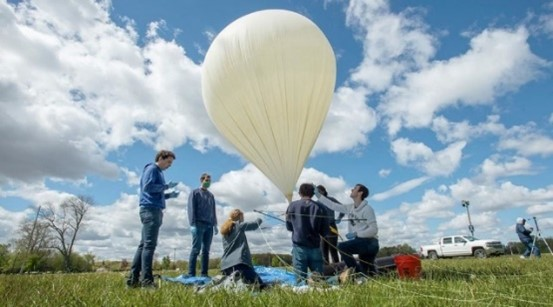
\includegraphics[width=.5\textwidth]{Pictures/HAB.jpg}
\caption{\emph{High Altitude Balloon}. Fuente: engineering.nd.edu }\label{fig:HAB}
\index{figures}
\end{figure}


\textbf{\emph{Zero-Pressure Balloons}:} Estos globos, con apertura en la parte inferior y conductos abiertos en los lados, permiten la liberación de gas y evitan el aumento de la presión interna a medida que se elevan. Sin embargo, su duración es limitada debido a la pérdida gradual de gas causada por el ciclo día/noche y las fluctuaciones de temperatura.

\begin{figure}[hbt!]
\centering
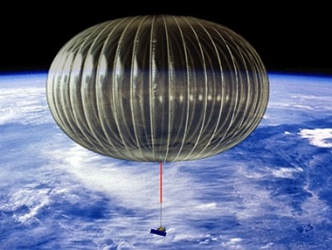
\includegraphics[width=.8\textwidth]{Pictures/ZeroP.png}
\caption{\emph{Zero-Pressure Balloon}. Fuente: https://stratocat.com.ar/ }\label{fig:ZeroP}
\index{figures}
\end{figure}

\textbf{\emph{Super-Pressure Balloons} (ULDB):} A diferencia de otros tipos de globos, en los ULDB el gas no puede escapar y la presión interna aumenta a medida que el gas se expande. Gracias a esta característica, la pérdida de gas en los globos de superpresión es mínima, lo que les permite volar durante períodos de tiempo más prolongados en comparación con los globos de presión cero.\\
Ambos tipos de globos no convencionales están hechos de polietileno, con un tamaño común de 40 millones de pies cúbicos. Se inflan con helio y pueden alcanzar una altitud de aproximadamente 120,000 pies, más del doble de la altitud de los aviones comerciales.


\begin{figure}[h!]
\centering
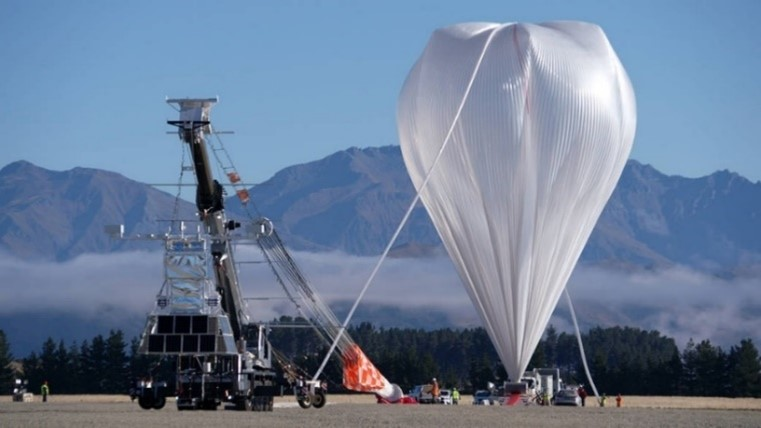
\includegraphics[width=.8\textwidth]{Pictures/SuperP.jpg}
\caption{\emph{Super-Pressure Balloon}. Fuente: nasa.gov }\label{fig:SuperP}
\index{figures}
\end{figure}

\newpage

Entre los logros más destacados se incluyen dos premios Nobel de Física, otorgados en 1936 y 2006, por el descubrimiento de los rayos cósmicos y el descubrimiento de la acelerada expansión del universo, respectivamente \cite{Nobel}.

\newpage


\section{Revisión del Estado del Arte de Sistemas de Eléctricos de Potencia (EPS) en aplicaciones de globos de gran altitud}

\vspace{0.5 cm}

Este trabajo se enfoca en el diseño y simulación de un sistema eléctrico de potencia (EPS) para misiones de corta duración con globos de gran altitud, priorizando la utilización de componentes electrónicos comerciales de bajo costo.

Al revisar la literatura, se observa la escasez de publicaciones directamente enfocadas en EPS para misiones con globos de gran altitud (HAB). Destacan trabajos, como el de la Universidad Sergio Arboleda en Colombia, que orienta el diseño de EPS para \emph{Balloonsats} y \emph{Cubesats} \cite{Vecino2013, comparasun,energiasat}, Estos trabajos se centran en modelos, simulación, experimentos y análisis exhaustivos de los componentes de un sistema de energía, abarcando celdas solares, baterías y convertidores DC-DC.


En las publicaciones, las aplicaciones de EPS están mayormente dirigidas a pequeños satélites, destacándose el estándar CubeSat. Proyectos del Kyushu Institute of Technology exhiben diseños que no solo cumplen con los requisitos de entrega de potencia, sino que también orientan el EPS hacia la recolección de datos, como voltaje, corriente y temperatura de baterías y paneles solares. El propósito es que esta información sea útil para comparativas de rendimiento y diagnóstico temprano de fallas \cite{jara2022orbit}. Asimismo, sobresale el proyecto Pycubed de la Universidad de Stanford, conocido por su programación totalmente en Python, su documentación y la utilización de componentes comerciales de bajo costo \cite{pycubed}.


Por otro lado, existen también diseños de EPS en aplicaciones híbridas de globos de gran altitud con CubeSat, como el proyecto TASEC-Lab de la Universidad Politécnica de Madrid. Este proyecto ejemplifica que los diseños con componentes comerciales para nanosatélites son aplicables para misiones de HAB, aplicándose de manera intercambiable. Además, el trabajo aborda factores ambientales relevantes para las misiones hacia la estratósfera, especialmente desde una perspectiva térmica en cada una de las capas previas. Se destaca una mención especial alrededor de los 11 km debido a una importante tasa de transferencia de calor por convección forzada. También se subraya la relevancia del control térmico pasivo con materiales como VDA, y se presentan pruebas ambientales en laboratorio, junto con un diseño simplificado de EPS que prioriza el funcionamiento y limita la complejidad innecesaria \cite{TASEC}.


Otros trabajos relevantes, aunque no centrados específicamente en EPS como un conjunto, abordan procesos relacionados. Destaca el trabajo de Eleazar Ramos en 2020, enfocado en la selección de baterías para nanosatélites según densidad energética, volumétrica y geometría \cite{Eleazar2020}. Revisiones exhaustivas sobre tecnología de baterías para misiones pequeñas, como la de Vaclav Knap en 2020, abordan criterios de selección, incluida la historia de vuelo y aplicaciones previas, junto con rigurosos procedimientos de pruebas para validar la seguridad de estas fuentes de almacenamiento de energía \cite{Knap2020}. Además, se encuentran estudios sobre el impacto térmico en el rendimiento de las baterías y la evolución con nuevos modelos, aspectos de alta relevancia para comprender las variables a controlar durante misiones en ambientes extremos \cite{Ma2018}.

En resumen, la revisión del estado del arte aporta modelos de arquitectura de EPS para aplicaciones desde vehículos eléctricos hasta nanosatélites, sin embargo, no se encuentran trabajos completos sobre el diseño de sistemas de energía para globos de gran altitud. Este vacío motiva el desarrollo de un EPS adaptado a las específicas condiciones de estas misiones para contribuir al avance de futuras investigaciones científicas que hagan uso de estas plataformas.

\newpage
\section{Metodología para el Diseño de Sistemas de Eléctricos de Potencia (EPS)}

\vspace{0.5 cm}

En relación a la metodología a implementar en este trabajo, la NASA ha establecido un ciclo de proyectos compuesto por siete fases, divididas en dos etapas fundamentales: formulación e implementación. La formulación abarca desde el estudio de conceptos hasta la completación tecnológica, mientras que la implementación se desarrolla desde el diseño final y fabricación hasta el cierre del proyecto, pasando por etapas cruciales como el ensamble, la integración y las pruebas \cite{NASA2016}. \\\\Además, el Modelo en V, ilustrado en la Fig. \ref{fig:fig_modelV}, ofrece una representación clara y coherente de esta metodología, aplicable específicamente al desarrollo de sistemas de energía para misiones de pequeños satélites \cite{IEEE_AESS_Distinguished_Lecture}. Dada la compatibilidad de este modelo con el enfoque de este trabajo, se considera prudente adoptarlo como una metodología con un historial probado en implementación.

\vspace{0.5 cm}

\begin{figure}[h]
  \centering
  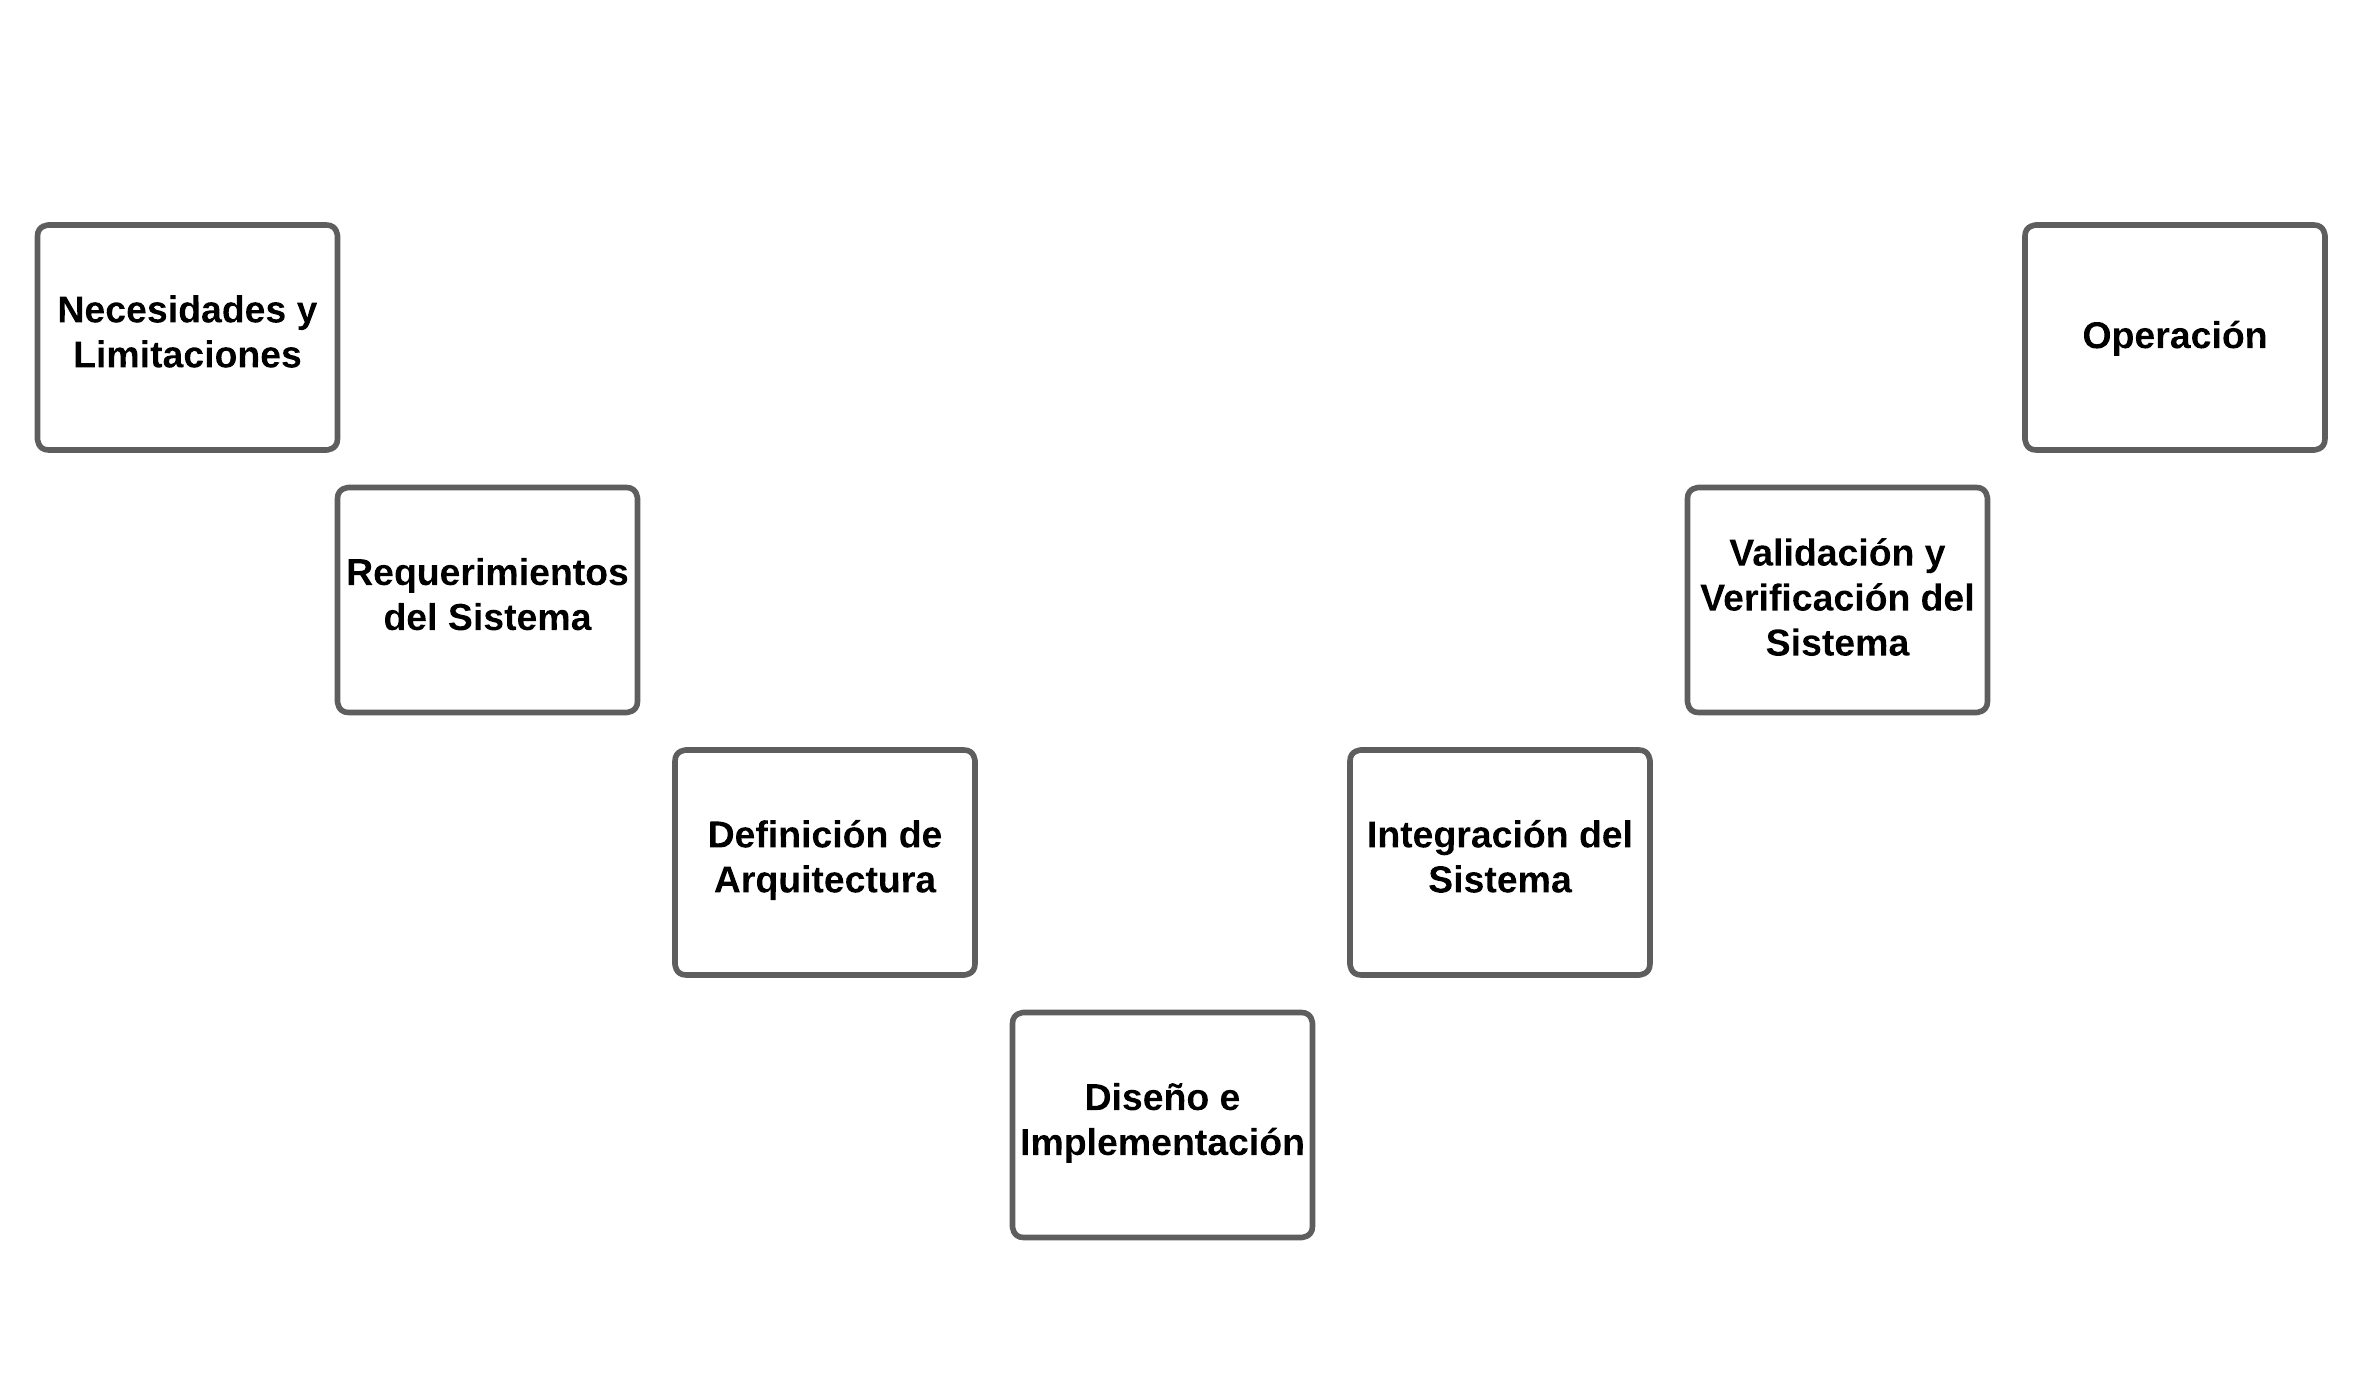
\includegraphics[width=\linewidth]{Pictures/ModeloV.png}
  \caption{Fases del modelo en V}
  \label{fig:fig_modelV}
\end{figure}


\subsection{Necesidades y Limitaciones}

En esta etapa, se busca caracterizar el sistema en función de su contexto de aplicación. Se identifican necesidades cruciales, como la resistencia a factores ambientales y la gestión eficiente del presupuesto energético. Además, se consideran las limitaciones específicas que el sistema debe abordar para adaptarse a las distintas condiciones de cada misión.

\subsection{Requerimientos del Sistema}

En esta fase, se concretizan las necesidades y limitaciones en una tabla de requerimientos. Es fundamental que estos estén claramente descritos, debidamente justificados y que cuenten con mecanismos de verificación medibles.

\subsection{Arquitectura}

Durante esta etapa, abordamos el diseño del sistema con un enfoque Top-Down, descomponiéndolo hasta alcanzar la mínima unidad funcional. Esto nos proporciona una comprensión detallada de la conexión y función conjunta de cada parte, sirviendo como base para las fases posteriores de integración. En esta fase, se detallan las entradas y salidas, tanto para el sistema en su vista más general como para cada una de sus subpartes.

\subsection{Diseño e Implementación}

En esta fase, transitamos del diseño funcional a la implementación física. Aquí, se realiza la selección de componentes en función de los requerimientos del sistema y de la arquitectura establecida. Se detallan las conexiones físicas a nivel de cada componente, definidas en el nivel más alto alcanzado en la arquitectura.

\subsection{Integración del Sistema}

La fase de integración comprende un proceso tanto a nivel de hardware como de software, con el objetivo de materializar el diseño funcional propuesto en la arquitectura.

\subsection{Validación y Verificación del Sistema}

En esta etapa, se define un plan de pruebas necesario para validar, a través de mediciones, que los requerimientos previamente establecidos se hayan alcanzado de manera efectiva.

\subsection{Operación}

Esta fase representa el punto culminante, donde el sistema integrado, validado y verificado, es puesto en funcionamiento en su entorno operativo.
 










